\documentclass{article}\usepackage[]{graphicx}\usepackage[]{color}
%% maxwidth is the original width if it is less than linewidth
%% otherwise use linewidth (to make sure the graphics do not exceed the margin)
\makeatletter
\def\maxwidth{ %
  \ifdim\Gin@nat@width>\linewidth
    \linewidth
  \else
    \Gin@nat@width
  \fi
}
\makeatother

\definecolor{fgcolor}{rgb}{0.345, 0.345, 0.345}
\newcommand{\hlnum}[1]{\textcolor[rgb]{0.686,0.059,0.569}{#1}}%
\newcommand{\hlstr}[1]{\textcolor[rgb]{0.192,0.494,0.8}{#1}}%
\newcommand{\hlcom}[1]{\textcolor[rgb]{0.678,0.584,0.686}{\textit{#1}}}%
\newcommand{\hlopt}[1]{\textcolor[rgb]{0,0,0}{#1}}%
\newcommand{\hlstd}[1]{\textcolor[rgb]{0.345,0.345,0.345}{#1}}%
\newcommand{\hlkwa}[1]{\textcolor[rgb]{0.161,0.373,0.58}{\textbf{#1}}}%
\newcommand{\hlkwb}[1]{\textcolor[rgb]{0.69,0.353,0.396}{#1}}%
\newcommand{\hlkwc}[1]{\textcolor[rgb]{0.333,0.667,0.333}{#1}}%
\newcommand{\hlkwd}[1]{\textcolor[rgb]{0.737,0.353,0.396}{\textbf{#1}}}%

\usepackage{framed}
\makeatletter
\newenvironment{kframe}{%
 \def\at@end@of@kframe{}%
 \ifinner\ifhmode%
  \def\at@end@of@kframe{\end{minipage}}%
  \begin{minipage}{\columnwidth}%
 \fi\fi%
 \def\FrameCommand##1{\hskip\@totalleftmargin \hskip-\fboxsep
 \colorbox{shadecolor}{##1}\hskip-\fboxsep
     % There is no \\@totalrightmargin, so:
     \hskip-\linewidth \hskip-\@totalleftmargin \hskip\columnwidth}%
 \MakeFramed {\advance\hsize-\width
   \@totalleftmargin\z@ \linewidth\hsize
   \@setminipage}}%
 {\par\unskip\endMakeFramed%
 \at@end@of@kframe}
\makeatother

\definecolor{shadecolor}{rgb}{.97, .97, .97}
\definecolor{messagecolor}{rgb}{0, 0, 0}
\definecolor{warningcolor}{rgb}{1, 0, 1}
\definecolor{errorcolor}{rgb}{1, 0, 0}
\newenvironment{knitrout}{}{} % an empty environment to be redefined in TeX

\usepackage{alltt}
\usepackage{geometry}
\geometry{verbose,tmargin=2cm,bmargin=2cm,lmargin=2.5cm,rmargin=2.5cm}
\IfFileExists{upquote.sty}{\usepackage{upquote}}{}
\begin{document}





\title{WA State HIV Testing Histories - Comparison of MSM-WA and MSM-KC}
\author{Martina Morris and Jeanette Birnbaum}
\maketitle

\section{Samples}




\paragraph{WA Sample}
\begin{itemize}
    \item N = 3135
    \item Years = 2005 to 2013
    \item everHadNegTest = TRUE for 1746 (55.69\%), FALSE for 301 (9.6\%), and NA for 1088 (34.7\%)
\end{itemize}

\paragraph{KC Sample}
\begin{itemize}
    \item N = 1522
    \item Years = 2006 to 2012
    \item everTested = TRUE for 1151 (75.62\%), FALSE for 101 (6.64\%), and NA for 270 (17.74\%)
\end{itemize}

Note on KC sample: in the Venn Diagram where I double-checked the revised Table 1 numbers, I found 1132 with a negative test and 289 with no testing history. I'm not sure why the data-cleaning.R file turns everTested=TRUE for 19 of those cases and we get 1151 flagged as having a negative test. Will have to investigate. Below when we look at the TID variable ('infPeriod'), it is NA for 289 cases, as we would expect. So, it looks like the everTested=TRUE flag is just wrong for those 19 cases, which shouldn't affect the results.

\section{TIDs}




\begin{knitrout}\footnotesize
\definecolor{shadecolor}{rgb}{0.969, 0.969, 0.969}\color{fgcolor}\begin{kframe}
\begin{alltt}
\hlkwd{summarize_infPeriod}\hlstd{(all}\hlopt{$}\hlstd{infPeriod,} \hlkwc{bygroup} \hlstd{= all}\hlopt{$}\hlstd{Population)}
\end{alltt}
\begin{verbatim}
## $stats
##   Group Min. 1st Qu. Median  Mean 3rd Qu.  Max. IsNA    N Percent Missing
## 1    KC    0  0.4986  1.249 3.119   3.332 17.98  289 1522           18.99
## 2    WA    0  0.5110  1.419 4.002   4.729 17.98 1088 3135           34.70
## 
## $oneway
## 
## 	One-way analysis of means (not assuming equal variances)
## 
## data:  infPeriod and Group
## F = 25.1526, num df = 1.000, denom df = 2994.363, p-value = 5.606e-07
\end{verbatim}
\end{kframe}
\end{knitrout}


\begin{knitrout}\footnotesize
\definecolor{shadecolor}{rgb}{0.969, 0.969, 0.969}\color{fgcolor}\begin{figure}[h]


{\centering 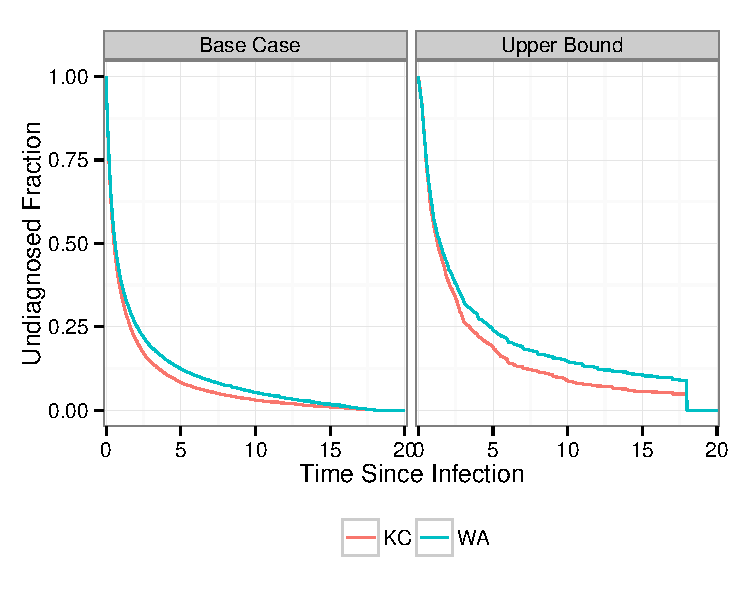
\includegraphics[width=\maxwidth]{figure/minimal-compare_TID_2} 

}

\caption[Time from infection to diagnosis (TID) for MSM, with panels representing difference cases (Base vs Upper Bound) and colors distinguishing populations (KC vs WA)]{Time from infection to diagnosis (TID) for MSM, with panels representing difference cases (Base vs Upper Bound) and colors distinguishing populations (KC vs WA)\label{fig:compare_TID_2}}
\end{figure}


\end{knitrout}


Figure \ref{fig:compare_TID_2} compares the TIDs for MSM in KC (red) versus MSM in WA (green). Both the Base Case (left) and Upper Bound (right) exclude those with TID=NA from the computation of TID, just as in the paper.
\section{Incidence and Undiagnosed Cases}

















\subsection{Summary across quarters, KC}
\begin{knitrout}\footnotesize
\definecolor{shadecolor}{rgb}{0.969, 0.969, 0.969}\color{fgcolor}\begin{kframe}
\begin{alltt}
\hlcom{# KC - replicates paper}
\hlstd{summaries_noimpute_KC[[}\hlnum{1}\hlstd{]]}
\end{alltt}
\begin{verbatim}
##                           var   Min. 1st Qu. Median   Mean 3rd Qu.   Max.
## 1               # Diagnosed    36.00   50.00  54.00  54.36   60.00  70.00
## 2     Incidence (Base Case)    49.73   53.15  54.88  54.29   55.61  57.53
## 3   Incidence (Upper Bound)    49.63   52.10  55.29  54.11   55.81  56.83
## 4   Undiagnosed (Base Case)   333.50  340.30 344.60 346.80  351.00 367.80
## 5 Undiagnosed (Upper Bound)   662.20  674.40 682.90 684.00  690.80 713.30
\end{verbatim}
\end{kframe}
\end{knitrout}


Replication of the paper results confirms that the code is working correctly.
\subsection{Summary across quarters, WA}
\begin{knitrout}\footnotesize
\definecolor{shadecolor}{rgb}{0.969, 0.969, 0.969}\color{fgcolor}\begin{kframe}
\begin{alltt}
\hlcom{# WA - using same code as the code that replicates the paper, this is what we get:}
\hlstd{summaries_noimpute_WA[[}\hlnum{1}\hlstd{]]}
\end{alltt}
\begin{verbatim}
##                           var    Min. 1st Qu.  Median    Mean 3rd Qu.    Max.
## 1               # Diagnosed     65.00   79.00   87.50   87.08   94.25  108.00
## 2     Incidence (Base Case)     75.75   81.27   87.99   85.40   89.94   90.47
## 3   Incidence (Upper Bound)     74.45   78.65   86.11   83.82   88.74   90.08
## 4   Undiagnosed (Base Case)    672.20  705.50  731.00  721.00  739.90  750.70
## 5 Undiagnosed (Upper Bound)   1341.00 1389.00 1445.00 1424.00 1459.00 1473.00
\end{verbatim}
\end{kframe}
\end{knitrout}






\clearpage
\subsection{Reported prevalence, undiagnosed counts, true prevalence, and the undiagnosed fraction}

In this table, UndiagQtrMin and UndiagQtrMax give the min-max range of quarterly undiagnosed counts across the quarters of one year, for a given Case and Population. TruePrevMin and TruePrevMax are the sum of ReportedPrev and the Min/Max UndiagQtr counts. UndiagPercMin and UndiagPercMax are the Min/Max of UndiagQtr divided by the Min/Max of TruePrev, converted to percents. 

\begin{knitrout}\footnotesize
\definecolor{shadecolor}{rgb}{0.969, 0.969, 0.969}\color{fgcolor}\begin{kframe}
\begin{alltt}
\hlstd{yearlys5}
\end{alltt}
\begin{verbatim}
##    Population          Category Group Year          Case Reported_Prev UndiagQtrMax UndiagQtrAvg
## 1          KC Mode-consolidated   MSM 2006   Base Case            5516        347.7        344.8
## 2          KC Mode-consolidated   MSM 2007   Base Case            5516        351.5        343.9
## 3          KC Mode-consolidated   MSM 2008   Base Case            5516        349.4        345.0
## 4          KC Mode-consolidated   MSM 2009   Base Case            5516        367.8        361.0
## 5          KC Mode-consolidated   MSM 2010   Base Case            5516        366.5        355.3
## 6          KC Mode-consolidated   MSM 2011   Base Case            5516        344.0        342.1
## 7          KC Mode-consolidated   MSM 2012   Base Case            5516        339.0        335.8
## 8          KC Mode-consolidated   MSM 2006 Upper Bound            5516        687.3        683.4
## 9          KC Mode-consolidated   MSM 2007 Upper Bound            5516        689.8        680.8
## 10         KC Mode-consolidated   MSM 2008 Upper Bound            5516        693.7        687.1
## 11         KC Mode-consolidated   MSM 2009 Upper Bound            5516        713.3        707.6
## 12         KC Mode-consolidated   MSM 2010 Upper Bound            5516        707.3        691.2
## 13         KC Mode-consolidated   MSM 2011 Upper Bound            5516        675.9        672.9
## 14         KC Mode-consolidated   MSM 2012 Upper Bound            5516        668.4        664.9
## 15         WA Mode-consolidated   MSM 2005   Base Case            7063        744.5        739.3
## 16         WA Mode-consolidated   MSM 2006   Base Case            7373        747.6        743.6
## 17         WA Mode-consolidated   MSM 2007   Base Case            7655        750.7        735.6
## 18         WA Mode-consolidated   MSM 2008   Base Case            7871        740.2        733.3
## 19         WA Mode-consolidated   MSM 2009   Base Case            8075        743.3        740.3
## 20         WA Mode-consolidated   MSM 2010   Base Case            8308        739.8        727.8
## 21         WA Mode-consolidated   MSM 2011   Base Case            8291        715.4        708.3
## 22         WA Mode-consolidated   MSM 2012   Base Case            8367        699.0        686.1
## 23         WA Mode-consolidated   MSM 2013   Base Case            8673        680.1        674.9
## 24         WA Mode-consolidated   MSM 2005 Upper Bound            7063       1470.9       1465.4
## 25         WA Mode-consolidated   MSM 2006 Upper Bound            7373       1473.0       1468.4
## 26         WA Mode-consolidated   MSM 2007 Upper Bound            7655       1471.9       1452.8
## 27         WA Mode-consolidated   MSM 2008 Upper Bound            7871       1458.4       1450.5
## 28         WA Mode-consolidated   MSM 2009 Upper Bound            8075       1458.5       1452.9
## 29         WA Mode-consolidated   MSM 2010 Upper Bound            8308       1444.2       1426.1
## 30         WA Mode-consolidated   MSM 2011 Upper Bound            8291       1404.2       1393.5
## 31         WA Mode-consolidated   MSM 2012 Upper Bound            8367       1376.2       1359.5
## 32         WA Mode-consolidated   MSM 2013 Upper Bound            8673       1349.4       1343.8
##    UndiagQtrMin TruePrevMin TruePrevAvg TruePrevMax UndiagPercMin UndiagPercAvg UndiagPercMax
## 1         339.5      5855.5      5860.8      5863.7           5.8           5.9           5.9
## 2         337.1      5853.1      5859.9      5867.5           5.8           5.9           6.0
## 3         342.1      5858.1      5861.0      5865.4           5.8           5.9           6.0
## 4         353.1      5869.1      5877.0      5883.8           6.0           6.1           6.3
## 5         345.7      5861.7      5871.3      5882.5           5.9           6.1           6.2
## 6         340.5      5856.5      5858.1      5860.0           5.8           5.8           5.9
## 7         333.5      5849.5      5851.8      5855.0           5.7           5.7           5.8
## 8         678.7      6194.7      6199.4      6203.3          11.0          11.0          11.1
## 9         674.9      6190.9      6196.8      6205.8          10.9          11.0          11.1
## 10        682.1      6198.1      6203.1      6209.7          11.0          11.1          11.2
## 11        700.3      6216.3      6223.6      6229.3          11.3          11.4          11.5
## 12        678.0      6194.0      6207.2      6223.3          10.9          11.1          11.4
## 13        671.2      6187.2      6188.9      6191.9          10.8          10.9          10.9
## 14        662.2      6178.2      6180.9      6184.4          10.7          10.8          10.8
## 15        735.6      7798.6      7802.3      7807.5           9.4           9.5           9.5
## 16        739.4      8112.4      8116.6      8120.6           9.1           9.2           9.2
## 17        723.9      8378.9      8390.6      8405.7           8.6           8.8           8.9
## 18        728.7      8599.7      8604.3      8611.2           8.5           8.5           8.6
## 19        737.5      8812.5      8815.3      8818.3           8.4           8.4           8.4
## 20        719.0      9027.0      9035.8      9047.8           8.0           8.1           8.2
## 21        705.2      8996.2      8999.3      9006.4           7.8           7.9           7.9
## 22        677.5      9044.5      9053.1      9066.0           7.5           7.6           7.7
## 23        672.2      9345.2      9347.9      9353.1           7.2           7.2           7.3
## 24       1460.8      8523.8      8528.4      8533.9          17.1          17.2          17.2
## 25       1464.5      8837.5      8841.4      8846.0          16.6          16.6          16.7
## 26       1440.0      9095.0      9107.8      9126.9          15.8          16.0          16.1
## 27       1446.7      9317.7      9321.5      9329.4          15.5          15.6          15.6
## 28       1449.8      9524.8      9527.9      9533.5          15.2          15.2          15.3
## 29       1412.3      9720.3      9734.1      9752.2          14.5          14.7          14.8
## 30       1386.7      9677.7      9684.5      9695.2          14.3          14.4          14.5
## 31       1349.1      9716.1      9726.5      9743.2          13.9          14.0          14.1
## 32       1340.7     10013.7     10016.8     10022.4          13.4          13.4          13.5
\end{verbatim}
\end{kframe}
\end{knitrout}


\begin{knitrout}\footnotesize
\definecolor{shadecolor}{rgb}{0.969, 0.969, 0.969}\color{fgcolor}\begin{kframe}
\begin{alltt}
\hlkwd{ddply}\hlstd{(yearlys5,} \hlkwd{.}\hlstd{(Population, Case),} \hlkwd{numcolwise}\hlstd{(range))}
\end{alltt}
\begin{verbatim}
##   Population          Case Year Reported_Prev UndiagQtrMax UndiagQtrAvg UndiagQtrMin TruePrevMin
## 1         KC   Base Case   2006          5516        339.0        335.8        333.5      5849.5
## 2         KC   Base Case   2012          5516        367.8        361.0        353.1      5869.1
## 3         KC Upper Bound   2006          5516        668.4        664.9        662.2      6178.2
## 4         KC Upper Bound   2012          5516        713.3        707.6        700.3      6216.3
## 5         WA   Base Case   2005          7063        680.1        674.9        672.2      7798.6
## 6         WA   Base Case   2013          8673        750.7        743.6        739.4      9345.2
## 7         WA Upper Bound   2005          7063       1349.4       1343.8       1340.7      8523.8
## 8         WA Upper Bound   2013          8673       1473.0       1468.4       1464.5     10013.7
##   TruePrevAvg TruePrevMax UndiagPercMin UndiagPercAvg UndiagPercMax
## 1      5851.8      5855.0           5.7           5.7           5.8
## 2      5877.0      5883.8           6.0           6.1           6.3
## 3      6180.9      6184.4          10.7          10.8          10.8
## 4      6223.6      6229.3          11.3          11.4          11.5
## 5      7802.3      7807.5           7.2           7.2           7.3
## 6      9347.9      9353.1           9.4           9.5           9.5
## 7      8528.4      8533.9          13.4          13.4          13.5
## 8     10016.8     10022.4          17.1          17.2          17.2
\end{verbatim}
\end{kframe}
\end{knitrout}


As in the paper, the undiagnosed fraction in KC MSM over 2006-2012 is 5.7-6.3 (BC) or 10.7-11.5 (UB). In MSM in WA over 2005-2013, the undiagnosed fraction is 7.2-9.5 (BC) or 13.4-17.2 (UB). 
\end{document}


